%File: anonymous-submission-latex-2026.tex
\documentclass{article}
\usepackage{iclr2027_conference,times}
\input{math_commands.tex}
\usepackage[hyphens]{url}
\usepackage{graphicx}
\usepackage{hyperref}
\usepackage{caption}
\usepackage{amsmath,amssymb}

\newcommand{\ours}{TreeMAPPO}
\newcommand{\toolflag}[1]{\textsc{#1}}

\title{TreeMAPPO: Fine-Grained Credit Assignment for Agentic LLM Training via Token-Level Trajectory Branching}

% Authors must not appear in the submitted version. They should be hidden
% as long as the \iclrfinalcopy macro remains commented out below.
% \iclrfinalcopy
\author{Anonymous Authors}

\begin{document}
\maketitle

\begin{abstract}
We present \ours, a reference-free framework for fine-grained credit assignment in agentic large language model training. Rather than assigning a single scalar reward to an entire reasoning trajectory, \ours\ constructs a rollout tree, estimates segment-level contribution from mixed-success leaves, and converts these estimates into dense token-level training signals. The method is designed for mathematical reasoning agents whose trajectories may interleave natural-language reasoning, fenced Python tool calls, tool responses, and final boxed answers. Compared with methods such as TEMPO that exploit shared prefixes among sampled trajectories, \ours\ actively creates new continuations through guided token-level branching, concentrating exploration at structurally useful and model-plausible decision points. Compared with TreeRPO-style tree credit assignment based on empirical outcome comparisons, \ours\ uses a statistically grounded maximum-a-posteriori posterior model that estimates signed segment contribution before producing token-level advantages. Experiments use a resource-efficient split pipeline that rolls out from the base policy, generates advantage-weighted training data, fine-tunes LoRA adapters, and validates checkpoint snapshots. Current results show consistent but modest validation gains across several model families, stronger gains in some tool-use settings, and mixed transfer to broader held-out tests.
\end{abstract}

\section{Introduction}
Sparse end-of-trajectory supervision makes credit assignment a central bottleneck in reinforcement learning for reasoning agents. When a long rollout contains many reasoning tokens, optional tool calls, and only a terminal correctness judgment, a single trajectory-level reward provides little guidance about which intermediate decisions should be reinforced or suppressed. The difficulty is especially acute in agentic settings, where early errors may be repaired by later reasoning or external tool feedback.

Recent work has begun to exploit shared-prefix and tree structure to densify supervision, including implicit prefix-tree methods, explicit tree-sampling methods, off-policy prefix-aware methods, and fine-grained agentic branching methods \cite{tempo2025,treerpo2025,treepo2025,treeopo2025,appo2026}. These methods show that branching structure exposes local comparisons that are unavailable to flat rollout groups. However, existing approaches often rely on naturally occurring prefix overlap, fixed segment boundaries, offline teacher-generated trees, or heuristic credit estimators that do not explicitly represent uncertainty.

This paper develops fine-grained credit assignment for mathematical reasoning agents through token-level trajectory branching. The central idea is to turn a small set of full rollouts into a structured tree of alternative continuations, then infer which segments are helpful, harmful, or uncertain from the pattern of correct and incorrect descendants. We call the resulting method \ours\ (Tree-based Maximum-A-Posteriori Policy Optimization).

Our implementation uses a lightweight tool-calling protocol: the model receives a question and an optional Python tool specification, emits reasoning in text, may invoke the tool via fenced Python markdown blocks, observes the tool response in context, and is required to terminate with a final answer wrapped in \texttt{\textbackslash boxed\{\}}. Rollouts are organized into trees, branch points are chosen at token granularity, and segment-level posterior estimates are transformed into token-level training advantages. The experiments in this submission emphasize a split one-shot pipeline: collect rollouts from the base model, construct the training set once for each condition, train adapters for multiple epochs, and validate the resulting checkpoints. This isolates the proposed credit-assignment mechanism while keeping the compute budget tractable.

Our contributions are:
\begin{itemize}
    \item We formulate fine-grained credit assignment as posterior inference over signed segment contributions in a trajectory tree.
    \item We introduce a guided branching policy that prioritizes model-plausible token-level alternatives while discouraging over-fragmentation and over-concentration, with forced first-token branching used to make the intended alternative explicit.
    \item We describe a practical training pipeline that converts rollout trees into non-redundant training trajectories with token-level advantages.
    \item We report split-pipeline LoRA experiments showing small positive validation gains in Qwen2.5-7B and Qwen3-4B settings, together with negative results that identify instability at overly aggressive learning rates and mixed held-out transfer.
\end{itemize}

\begin{figure}[t]
\centering
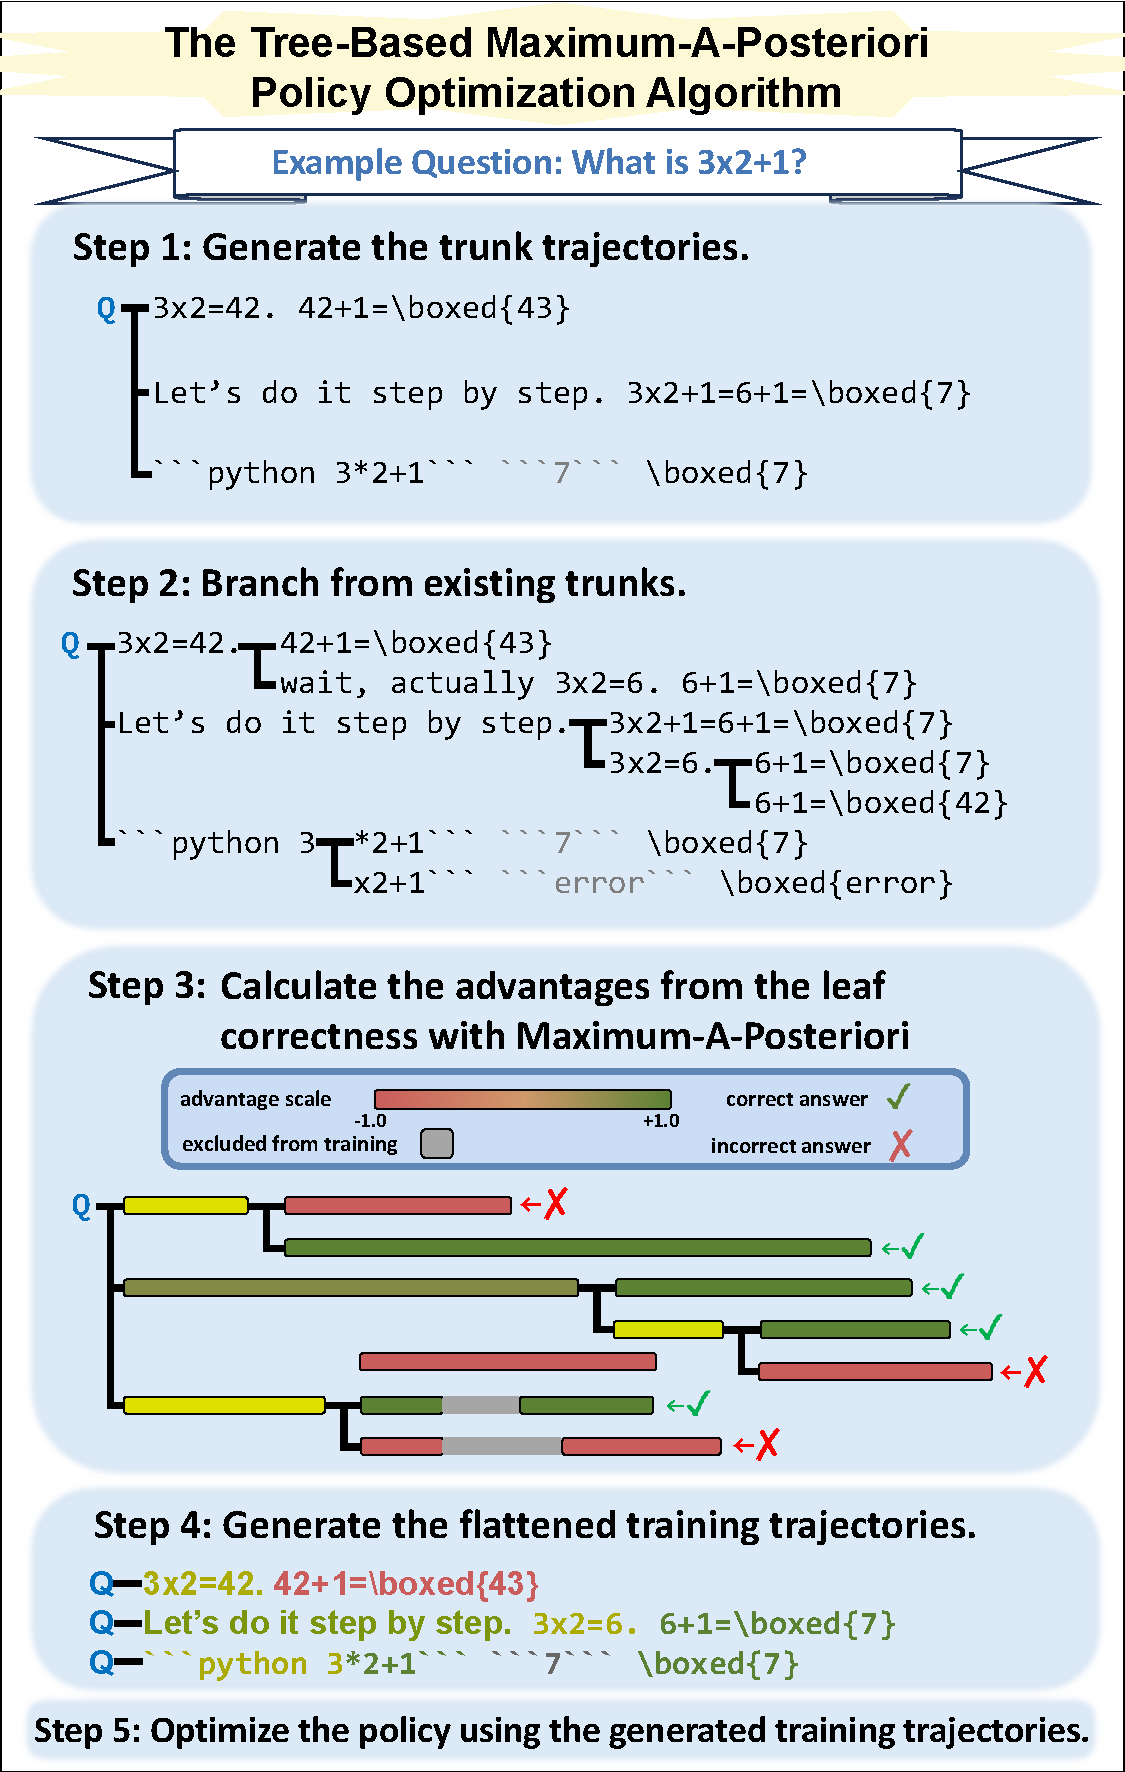
\includegraphics[width=\textwidth]{images/tree_mappo_methodology.pdf}
\caption{Method overview. \ours\ samples base-policy trajectories, expands selected token-level branch points, infers segment-level contribution and uncertainty from leaf correctness, and converts the resulting posterior estimates into token-level advantages for adapter training.}
\label{fig:methodology}
\end{figure}

\section{Related Work}
\paragraph{Trajectory-level RL for reasoning.}
Reinforcement learning with verifiable rewards has become a standard recipe for improving mathematical and agentic reasoning, because final-answer correctness can often be checked automatically. PPO remains a canonical policy-optimization baseline: it stabilizes policy updates with a clipped surrogate objective and obtains token-level advantages through a learned value function \cite{ppo17}. GRPO, introduced in DeepSeekMath, removes the critic by normalizing outcome rewards within groups of sampled responses, substantially reducing training complexity while retaining the appeal of verifiable rewards \cite{deepseekmath2024}. The limitation of both trajectory-level and group-relative outcome supervision is the one targeted here: when a long response receives only terminal feedback, many irrelevant tokens are reinforced or suppressed together with the decisive reasoning steps.

\paragraph{Process supervision and verifier-based credit.}
A complementary line of work makes supervision denser by judging intermediate reasoning steps. Let’s Verify Step by Step showed that process supervision can outperform outcome-only supervision on mathematical reasoning by training process reward models from step-level human labels \cite{lightman2023letsverify}. This line establishes the value of fine-grained credit, but it changes the supervision regime: it depends on annotated intermediate labels, learned verifiers, or additional reward-model infrastructure. \ours\ instead keeps the outcome-only setting and infers local credit from the structure of sampled rollouts. The distinction is important methodologically: our goal is not to build a stronger verifier, but to convert sparse terminal correctness into localized training signals without step-level references.

\paragraph{Implicit tree and shared-prefix methods.}
TEMPO \cite{tempo2025} converts a group of sampled responses into a prefix tree and adds branch-gated temporal-difference corrections on top of a GRPO-style training loop. Its main appeal is that it preserves a relatively simple rollout interface while extracting token-level signal where natural branching occurs. Our method differs in that we do not rely on incidental prefix overlap alone; instead, we explicitly create new branches at selected token positions, which provides direct control over branching density using rollout structure and model-side alternative-token probabilities.

\paragraph{Explicit tree sampling and tree-aware advantages.}
TreeRPO \cite{treerpo2025} and TreePO \cite{treepo2025} both pursue explicit tree-structured sampling to obtain denser supervision. TreeRPO estimates step-level reward expectations via tree sampling and forms step-level comparison groups without a separate reward model. TreePO emphasizes systems efficiency, shared-prefix reuse, and subgroup-relative advantages over segment-level trees. Our method is closest in spirit to this line, but differs in two important respects: first, we branch at arbitrary token positions rather than imposing fixed step or segment partitions; second, we infer segment contribution with a probabilistic MAP model that explicitly represents uncertainty, rather than relying only on win-rate or subgroup heuristics.

\paragraph{Prefix-aware and off-policy tree supervision.}
Tree-OPO \cite{treeopo2025} uses teacher-generated MCTS prefixes and staged advantage estimation to create prefix-aware off-policy training groups. By contrast, \ours\ is on-policy and reference-free: the tree is constructed directly from the policy's own rollouts, without offline teacher trees, reward models, or process-level supervision.

\paragraph{Agentic RL and branching granularity.}
APPO \cite{appo2026} studies branching and credit assignment in tool-using agents, arguing that influential decision points are not confined to tool-call boundaries or coarse workflow stages. This observation aligns closely with our setting. The main methodological difference is that APPO uses a branching score and procedure-level advantage scaling, whereas \ours\ combines explicit token-level branching with posterior inference over signed segment contribution and uncertainty.

\paragraph{Tool-augmented mathematical reasoning and benchmarks.}
Our agent protocol is also related to work on tool-augmented reasoning. PAL and Program-of-Thoughts showed that language models can delegate arithmetic or symbolic computation to Python programs, improving numerical reasoning by separating decomposition from execution \cite{gao2022pal,chen2022pot}. ReAct generalized interleaved reasoning and acting, while Toolformer studied how models can learn tool use from limited demonstrations \cite{yao2022react,schick2023toolformer}. These methods motivate the mixed text--tool trajectories considered here, but they primarily address inference-time tool use rather than training-time credit assignment. Our evaluation setting builds on mathematical reasoning resources such as MATH \cite{hendrycks2021math} and recent verifiable training corpora such as DeepMath-103K \cite{he2025deepmath103k}; the broader benchmark mix is intended to test whether tree-based credit assignment transfers beyond the distribution used to construct training trajectories.

\begin{figure}[t]
\centering
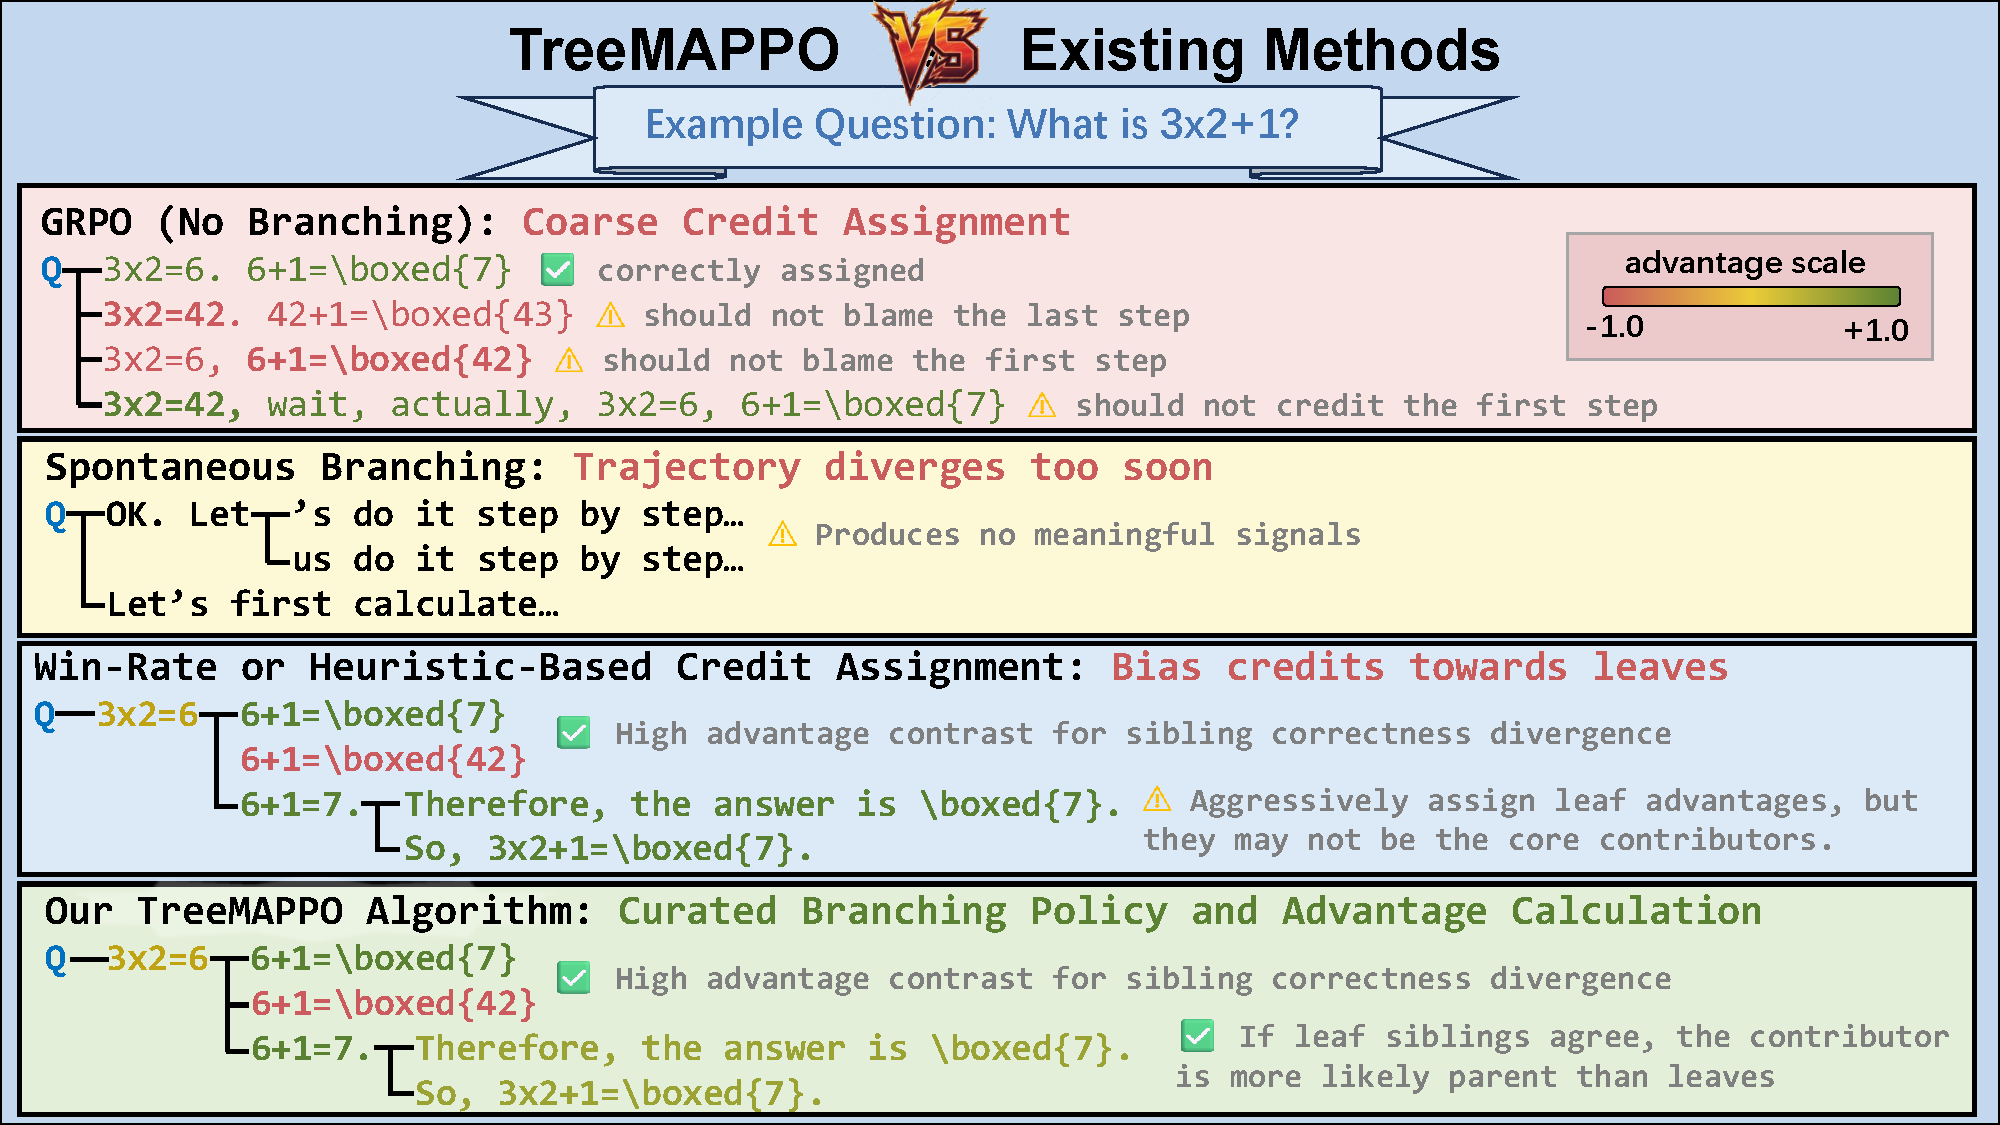
\includegraphics[width=\textwidth]{images/tree_mappo_comparison.pdf}
\caption{Comparison of credit-assignment structures. Trajectory-level GRPO assigns one normalized outcome signal to every token; TEMPO extracts branch-gated corrections from natural shared prefixes; TreeRPO uses fixed-step tree sampling and empirical child-group rewards; \ours\ combines guided token-level branching with posterior segment-credit inference.}
\label{fig:method-comparison}
\end{figure}



\section{Problem Setting and Agent Protocol}
We study question-answering agents for mathematical reasoning. Each sample provides a problem statement and a ground-truth final answer used only for post hoc correctness judgment. During rollout, the model may produce plain-text reasoning and, when enabled, invoke a Python executor.

Our implementation uses the following protocol.
\begin{enumerate}
    \item Each prompt contains the problem statement and, when tool use is enabled, a specification that Python can be called by emitting a fenced markdown block.
    \item The model may interleave reasoning and tool use.
    \item When a fenced Python block closes, generation pauses, the tool executes, and the tool response is appended to the context.
    \item The model is instructed to present its final answer in \texttt{\textbackslash boxed\{\}}.
    \item If generation reaches a control handoff without a boxed answer, the framework requests continuation until a boxed answer is produced or rollout termination conditions are hit.
\end{enumerate}

This protocol is consistent across training-data collection and evaluation so that differences across methods are attributable to branching and credit assignment rather than prompt format changes.

\section{Method}
\subsection{Overview}
For each question, we first sample a set of complete trunk trajectories. We then expand a rollout tree by branching from selected token positions. Each completed leaf trajectory is judged as correct or incorrect using its extracted final boxed answer. The resulting leaf labels provide supervision for segment-level posterior inference. Posterior estimates are transformed into branching scores for future expansions and into training advantages for model optimization.

\subsection{Trajectory Tree Construction}
In the default configuration for our main tool-using setup, we begin with 4 trunk trajectories and expand to 16 total trajectories. Our experimental plan also includes branch-budget variants with 8 and 32 total trajectories.

Branching is token-level rather than step-level. A new branch can be created in two ways:
\begin{itemize}
    \item \textbf{Segment split:} split an existing reasoning segment at an internal token position and regenerate from that point.
    \item \textbf{Node expansion:} branch again from an existing branching node, increasing its branching factor.
\end{itemize}

The implementation keeps a fixed decoding temperature within each tree. In the current configs, this value is $T=0.7$ for trunk generation, continuation, and branch expansion.

\subsection{MAP Credit Assignment Model}
Let $\ell$ index judged leaves and let $i$ index non-prompt segments. For each leaf $\ell$:
\begin{itemize}
    \item $y_\ell \in \{+1,-1\}$ is the correctness label.
    \item $x_{\ell,i} \in \{0,1\}$ indicates whether segment $i$ lies on the path to leaf $\ell$.
    \item Segment $i$ has mean contribution $m_i$ and log standard deviation $u_i$.
\end{itemize}

Leaf-level moments are
\begin{align}
\mu_\ell &= \sum_i x_{\ell,i} m_i, \\
\tau_\ell &= \sqrt{\sum_i x_{\ell,i} \exp(2u_i) + \varepsilon}, \\
z_\ell &= y_\ell \mu_\ell / \tau_\ell.
\end{align}
We use a probit likelihood,
\begin{equation}
p(y_\ell \mid \{m_i,u_i\}) = \Phi(z_\ell),
\end{equation}
where $\Phi$ is the standard normal CDF.

Our implementation initializes prior means at zero and optimizes the negative log posterior
\begin{equation}
\mathcal{J} = -\sum_\ell \log \Phi(z_\ell)
+ \frac{1}{2\sigma_m^2}\sum_i m_i^2
+ \frac{1}{2\sigma_u^2}\sum_i u_i^2.
\end{equation}

The current hyperparameter file uses
$\sigma_m = 1.0$,
$\sigma_u = 1.0$,
$\varepsilon = 10^{-6}$,
120 optimization iterations, and log-standard-deviation clamps in $[-4,2]$.
Optimization is performed with gradient steps and backtracking line search, together with a numerically stable implementation of $\log \Phi$ for large negative margins.

\subsection{Guided Token-Level Branching}
The current implementation chooses branch points before leaf judgments are available. Branching therefore relies on rollout structure and model-side token statistics rather than posterior uncertainty. For each candidate token position, the implementation multiplies:
\begin{enumerate}
    \item a structural penalty, and
    \item the relative probability of the best alternative token that differs from the already-sampled continuation.
\end{enumerate}
Candidates whose best alternative has relative probability below $0.1$ are discarded.

For node expansion, the structural penalty is an exponential branching-factor penalty,
\begin{equation}
\gamma_{\text{node}}(b) = \exp\big(-k_{\text{node}}(b-1)\big),
\end{equation}
with $k_{\text{node}}=0.35$ in the current implementation.
For segment splitting, the structural penalty increases with the shorter side of the split relative to average trunk length, discouraging very short fragments.

After a branch point and alternative token are selected, the current guided-branching implementation forces that selected token to be the first token of the new branch continuation. This makes the token-level branch explicit rather than merely restarting generation from the shared prefix and hoping that sampling chooses the intended alternative. We keep the non-forced version as an ablation, but use the forced-token version as the default because it better matches the intended token-level intervention.

\subsection{From Posterior Scores to Training Advantages}
After tree construction, each segment receives an unnormalized signed score proportional to $m_i / \exp(u_i)$. The methodology notes propose an additional length-aware rescaling to reduce volatility from very short reasoning spans. The generated training samples then attach token-level advantage values aligned with the input sequence.

The downstream training code consumes aligned token sequences, supervised target tokens, attention masks, token-level advantages, and old token log probabilities. The loss is a clipped policy-ratio surrogate over supervised positions,
\begin{equation}
\mathcal{L}_{\text{train}} = -\frac{1}{|\mathcal{S}|}
\sum_{t \in \mathcal{S}}
\min\left(
\rho_t \tilde{A}_t,
\operatorname{clip}(\rho_t,1-\epsilon,1+\epsilon)\tilde{A}_t
\right),
\end{equation}
where $\mathcal{S}$ denotes supervised token positions, $\rho_t$ is the ratio between the current token probability and the stored old token probability, and $\tilde{A}_t$ is the token advantage clipped to $[-3,3]$. This is the implemented optimization interface for injecting segment-level credit into model updates while avoiding the unbounded negative-advantage objective that arises from direct advantage-weighted cross entropy.

\subsection{Training-Set Construction}
Because many tree leaves share prefixes, naively flattening all leaves would over-train shared segments. We therefore use a greedy de-duplication policy.
\begin{enumerate}
    \item Score each candidate leaf trajectory by average absolute token advantage.
    \item Select the strongest candidate.
    \item Mark its segments as consumed.
    \item Repeat among trajectories that still contain unconsumed learnable segments.
    \item Aggregate selected trajectories across trees and prune the tail with a cumulative average-absolute-advantage cutoff.
\end{enumerate}

Selected trajectories are finally ordered by a configurable batching policy. In length-based runs, this improves early memory stability; in by-question runs, it groups positive and negative samples from the same problem so the optimizer sees local contrasts consecutively.

\section{Baselines and Ablations}
We consider three primary comparison points.
\begin{itemize}
    \item \textbf{Base model:} no fine-tuning.
    \item \textbf{GRPO-style baseline:} use 8 trunks and 8 total trajectories, yielding multiple complete rollouts without token-level branching in the main tool setup.
    \item \textbf{\ours:} guided branching with MAP-based posterior credit assignment.
\end{itemize}

We also separate two ablation axes that are explicitly encoded in configs and scripts.
\begin{itemize}
    \item \textbf{TEMPO-style branching ablation:} switch the branching policy from guided branching to spontaneous divergence-point branching while keeping posterior-based credit assignment.
    \item \textbf{TreeRPO-style credit ablation:} keep guided branching but replace posterior-based segment advantages with bottom-up child-group outcome comparisons. For each branching group, terminal correctness is backed up into child subtree values; groups with negligible value spread are filtered; surviving children receive normalized relative advantages.
    \item \textbf{TreeRL-style branching ablation:} keep posterior-based credit assignment but select guided branch points by model entropy rather than our full branching score.
    \item \textbf{TreeRL-style credit ablation:} keep guided branching but replace posterior-based segment advantages with a local--global value-difference estimator, combining a segment's improvement over its parent with its improvement over the root.
\end{itemize}

In our implementation, these ablations are not merely renamed conditions: the TEMPO and TreeRL-branching ablations change the exploration rule, while the TreeRPO-style and TreeRL-credit ablations change the advantage-estimation rule. This distinction is important because it cleanly separates exploration structure from credit estimation.

\section{Experimental Setup}
\subsection{Models}
We evaluate the following model-condition families.
\begin{itemize}
    \item Qwen2.5-7B-Instruct with tool use.
    \item Qwen2.5-7B-Instruct without tool use.
    \item Qwen3-4B with tool use.
    \item Qwen3-4B without tool use.
    \item Gemma-3-4B-IT without tool use.
    \item Llama-3.1 and Mistral-7B without tool use.
\end{itemize}

For the main tables, tool-enabled and no-tool variants of the same backbone are treated as separate model-condition groups, since the prompting interface and action space differ.

\subsection{Datasets}
Training and validation are built from DeepMath, MATH, and NuminaMath.
\begin{itemize}
    \item The training JSONL file contains 5{,}000 samples per dataset, interleaved across the three in-distribution datasets.
    \item The validation JSONL file contains 1{,}000 validation samples per dataset drawn from disjoint index ranges after the training slice.
\end{itemize}

We also construct an aggregated held-out evaluation JSONL file from six datasets in this order: DeepMath, MATH, NuminaMath, AMC2023, GaoKao Math 2024, and CollegeMath. For datasets with more than 1{,}000 test rows, 1{,}000 are sampled with seed 42; for DeepMath, which lacks a dedicated test split in the current pipeline, evaluation rows are drawn from the training split after clearing the reserved training and validation examples.


\subsection{Training and Evaluation Protocol}
The primary experiments use a split one-shot protocol rather than a fully interleaved online reinforcement-learning loop. For each model-condition pair, we run four stages: base-policy rollout collection, training-set generation, adapter training, and checkpoint validation. Rollout and generation are performed once per condition using the base model, after which the generated trajectories and token-level advantages are reused across multiple LoRA training epochs. Validation then evaluates the base model and each trained checkpoint under the same inference protocol.

This protocol is intentionally different from a production online RL pipeline in which each epoch rolls out from the latest policy and immediately regenerates training data. The split protocol is less expensive, makes infrastructure failures easier to diagnose, and allows fair controlled comparisons among GRPO-style, TreeRPO-style, TEMPO-style, and \ours\ variants under the same rollout budget. When compute permits, the same codebase also supports a full orchestrator mode with repeated validation rollout, training rollout collection, training-set generation, and training across policy updates; those runs are treated as confirmatory rather than the main experimental path.

The training protocol uses the following recurring settings:
\begin{itemize}
    \item chunked one-shot training, where each epoch consumes one generated training chunk and recovery restarts at whole-chunk boundaries;
    \item LoRA rank 32 and learning rate $10^{-6}$ for the main stable runs, with Adam state and learning-rate warmup enabled unless stated otherwise;
    \item held-out validation at epoch 0 and then every 10 epochs for long runs, with multiple validation rollout trials used to reduce sampling noise;
    \item LoRA-based fine-tuning for the primary experiments, while full-model training is deferred because queueing and memory costs are substantially higher.
    \item fixed rollout temperature $0.7$.
\end{itemize}

The primary evaluation metric is pass@1 accuracy. Validation reports an equal-weight macro average over the in-distribution validation datasets. Serious testing uses a broader six-dataset mixture and reports an equal-weight macro average over datasets rather than over examples, so smaller datasets do not vanish in the aggregate.


\section{Results}
This section reports the audited experiment inventory available at submission time. All serious-test rows in the main tables use five rollout trials and all six test datasets; held-out validation rows use six trials. We emphasize conservative conclusions: the current evidence supports modest and repeatable validation improvements, but the broader serious tests show that these gains do not always transfer uniformly.

\subsection{Validation Accuracy Trends}
Table~\ref{tab:validation-results} summarizes audited held-out validation runs. ``Best'' is the best validated trained checkpoint, and gains are measured against the same run's base checkpoint. All listed training runs use single-GPU LoRA rank 32, learning rate $10^{-6}$, Adam, and warmup.

\begin{table}[t]
\centering
\resizebox{\textwidth}{!}{%
\begin{tabular}{llccccccc}
\hline
Model and condition & Method & Trials & Epochs audited & Base & Best epoch & Best & Gain & Last \\
\hline
Qwen2.5-7B no-tool & GRPO & 6 & 0,10,\ldots,70 & 0.6468 & 30 & 0.6538 & +0.0069 & 0.6522 \\
Qwen2.5-7B no-tool & \ours, forced token & 6 & 0,10,\ldots,70 & 0.6436 & 50 & 0.6523 & +0.0087 & 0.6494 \\
Qwen2.5-7B + tool & GRPO & 6 & 0,10,\ldots,70 & 0.6142 & 30 & 0.6246 & +0.0104 & 0.6171 \\
Qwen2.5-7B + tool & \ours, forced token & 6 & 0,10,\ldots,70 & 0.6134 & 50 & 0.6236 & +0.0101 & 0.6181 \\
Qwen3-4B no-tool & GRPO & 6 & 0,10,\ldots,50 & 0.6901 & 50 & 0.6991 & +0.0089 & 0.6991 \\
Qwen3-4B no-tool & \ours & 6 & 0,10,\ldots,50 & 0.6894 & 30 & 0.6944 & +0.0050 & 0.6849 \\
Qwen3-4B + tool & GRPO & 6 & 0,10,\ldots,50 & 0.6446 & 40 & 0.6617 & +0.0172 & 0.6521 \\
Qwen3-4B + tool & \ours & 6 & 0,10,\ldots,50 & 0.6434 & 50 & 0.6605 & +0.0171 & 0.6605 \\
Gemma-3-4B no-tool & GRPO & 6 & 0,10,\ldots,50 & 0.5640 & 50 & 0.5647 & +0.0007 & 0.5647 \\
Gemma-3-4B no-tool & \ours & 6 & 0,10,\ldots,50 & 0.5621 & 40 & 0.5643 & +0.0023 & 0.5594 \\
Mistral-7B no-tool & GRPO & 6 & 0,10,\ldots,50 & 0.1747 & 40 & 0.1802 & +0.0055 & 0.1729 \\
Mistral-7B no-tool & \ours & 6 & 0,10,\ldots,50 & 0.1747 & 10 & 0.1819 & +0.0072 & 0.1788 \\
Llama-3.1 no-tool & GRPO & 6 & 0,10,\ldots,50 & 0.4415 & 30 & 0.4684 & +0.0269 & 0.4609 \\
Llama-3.1 no-tool & \ours & 6 & 0,10,\ldots,40 & 0.4454 & 40 & 0.4589 & +0.0135 & 0.4589 \\
\hline
\end{tabular}%
}
\caption{Audited held-out validation results. Values are pass@1 macro averages on the validation mixture. All rows use six validation trials and epochs that are 0 or multiples of 10.}
\label{tab:validation-results}
\end{table}

Across validation runs, both GRPO and \ours\ extract usable signal from the split pipeline. Qwen2.5-7B gains are modest in both no-tool and tool settings, roughly one percentage point at the best audited checkpoints. Qwen3-4B shows stronger tool-use gains for both methods, and Llama-3.1 improves under GRPO before partially regressing. Gemma and Mistral remain weak in absolute accuracy, but their best checkpoints still show small positive validation movement. The main pattern is therefore not monotonic scaling with epoch count; checkpoint selection by validation is necessary.

\begin{figure}[t]
\centering
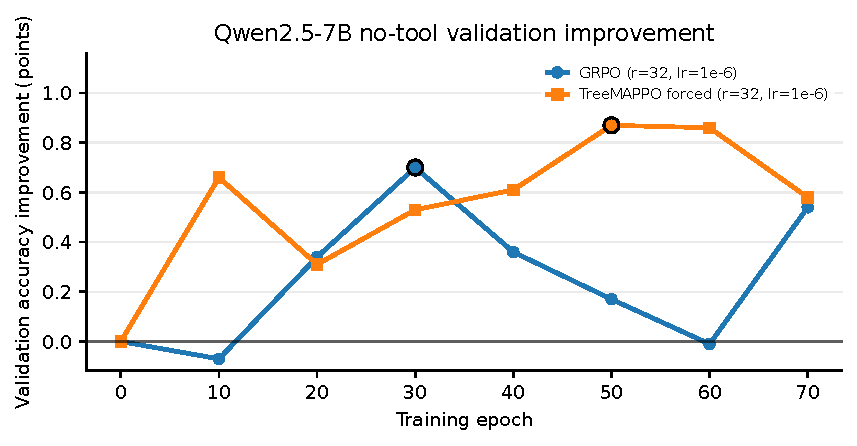
\includegraphics[width=\columnwidth]{images/qwen25_notool_epoch_improvement.pdf}
\caption{Validation accuracy improvement over the base checkpoint for Qwen2.5-7B in the no-tool setting. Both lines use LoRA rank 32 and learning rate $10^{-6}$; the y-axis reports percentage-point change relative to each method's epoch-0 validation accuracy.}
\label{fig:qwen25-notool-improvement}
\end{figure}

\subsection{Held-Out Serious Tests}
Table~\ref{tab:heldout-serious} reports serious tests on the broader six-dataset mixture. Each row uses the best checkpoint selected by validation for that method and setting, then evaluates it with five rollout trials. The macro average gives equal weight to datasets rather than to individual examples.

\begin{table}[t]
\centering
\resizebox{\textwidth}{!}{%
\begin{tabular}{llcccc}
\hline
Model and condition & Method & Epoch & Trials & Datasets & Macro avg. \\
\hline
Qwen2.5-7B no-tool & Base & 0 & 5 & 6 & 0.6366 \\
Qwen2.5-7B no-tool & GRPO & 30 & 5 & 6 & 0.6353 \\
Qwen2.5-7B no-tool & \ours, forced token & 50 & 5 & 6 & 0.6305 \\
Qwen2.5-7B + tool & Base & 0 & 5 & 6 & 0.5742 \\
Qwen2.5-7B + tool & GRPO & 30 & 5 & 6 & 0.5850 \\
Qwen2.5-7B + tool & \ours, forced token & 50 & 5 & 6 & 0.5836 \\
Qwen3-4B no-tool & Base & 0 & 5 & 6 & 0.6941 \\
Qwen3-4B no-tool & GRPO & 50 & 5 & 6 & 0.6999 \\
Qwen3-4B no-tool & \ours & 30 & 5 & 6 & 0.6997 \\
Qwen3-4B + tool & Base & 0 & 5 & 6 & 0.6255 \\
Qwen3-4B + tool & GRPO & 40 & 5 & 6 & 0.6487 \\
Qwen3-4B + tool & \ours & 50 & 5 & 6 & 0.6694 \\
Gemma-3-4B no-tool & Base & 0 & 5 & 6 & 0.5819 \\
Gemma-3-4B no-tool & GRPO & 50 & 5 & 6 & 0.5782 \\
Gemma-3-4B no-tool & \ours & 40 & 5 & 6 & 0.5906 \\
Mistral-7B no-tool & Base & 0 & 5 & 6 & 0.1664 \\
Mistral-7B no-tool & GRPO & 40 & 5 & 6 & 0.1674 \\
Mistral-7B no-tool & \ours & 20 & 5 & 6 & 0.1567 \\
Llama-3.1 no-tool & Base & 0 & 5 & 6 & 0.3926 \\
Llama-3.1 no-tool & GRPO & 30 & 5 & 6 & 0.4117 \\
Llama-3.1 no-tool & \ours & 40 & 5 & 6 & 0.4167 \\
\hline
\end{tabular}%
}
\caption{Held-out serious-test results. All rows use five rollout trials and six datasets. Epoch 0 denotes the base model; trained rows use the best validation-selected checkpoint available under the audited protocol.}
\label{tab:heldout-serious}
\end{table}

The serious tests sharpen the conclusion. In no-tool Qwen2.5-7B, neither trained method beats the base model on the six-dataset macro average despite validation gains, indicating limited transfer from the validation mixture. In tool-enabled Qwen2.5-7B, both trained methods improve over base by about one point, with GRPO and \ours\ close to each other. Qwen3-4B is the strongest positive setting: both methods improve in no-tool testing, and \ours\ substantially outperforms GRPO in the tool setting. Gemma and Llama provide additional positive evidence for \ours\ over their base models, while Mistral remains unstable and below base for \ours.

\subsection{Ablation Study}
The main ablation plan separates branching policy from credit estimation. The TEMPO-style condition changes the branch source to spontaneous shared-prefix divergence. The TreeRPO-style condition changes only the segment-credit estimator to child-group win-rate comparison. The two TreeRL-style conditions separately test entropy-guided branching and local--global value-difference credit. Guided-branching experiments use forced selected branch tokens by default; non-forced branching is retained only as a mechanism ablation.

\begin{table}[t]
\centering
\resizebox{\textwidth}{!}{%
\begin{tabular}{lcccccc}
\hline
Qwen2.5-7B no-tool variant & Best val. epoch & Val. base & Best val. & Val. gain & Test epoch & Test macro \\
\hline
GRPO baseline & 30 & 0.6468 & 0.6538 & +0.0069 & 30 & 0.6353 \\
\ours, non-forced token & 20 & 0.6439 & 0.6493 & +0.0054 & 20 & 0.6294 \\
\ours, forced token & 50 & 0.6436 & 0.6523 & +0.0087 & 50 & 0.6305 \\
TEMPO-style branching & 70 & 0.6392 & 0.6521 & +0.0129 & 70 & 0.6326 \\
TreeRPO-style credit & 40 & 0.6433 & 0.6520 & +0.0087 & 40 & 0.6272 \\
TreeRL-style branching & 20 & 0.6403 & 0.6490 & +0.0087 & 20 & 0.6195 \\
TreeRL-style credit & 60 & 0.6487 & 0.6523 & +0.0036 & 60 & 0.6334 \\
TreeRL combined & 40 & 0.6437 & 0.6522 & +0.0085 & 40 & 0.6341 \\
Branch budget 8 & 10 & 0.6434 & 0.6501 & +0.0067 & 10 & 0.6274 \\
Branch budget 32 & 60 & 0.6439 & 0.6509 & +0.0070 & 60 & 0.6333 \\
\hline
\end{tabular}
}
\caption{Qwen2.5-7B no-tool ablations. Validation numbers are held-out macro averages; testing uses five trials and six datasets. Ablation validation rows are directional when their validation trial count differs from the six-trial main rows, but their serious-test scores use the same five-trial testing protocol.}
\label{tab:ablation-results}
\end{table}

The ablations do not isolate a single universally dominant ingredient. TEMPO-style branching gives the largest validation gain among the ablations but does not beat GRPO or the strongest TreeRL-credit variants on serious testing. Forced branch tokens improve validation relative to the non-forced mechanism, which supports matching the sampled branch to the token probability used in the branch score, but the serious-test difference remains small. Branch budget also has no monotonic effect: the 32-trajectory variant beats the 8-trajectory variant on testing, but neither produces a large margin.

\subsection{Stability Diagnostics}
Several completed runs are negative results that shape the current claims. Qwen2.5-7B \ours\ at LoRA rank 32 with learning rate $5\times10^{-5}$ collapsed in earlier validation, while the same rank with learning rate $10^{-6}$ remained stable. SGD/no-warmup variants did not show useful trends and were removed from the main schedule. Mistral remains difficult under the current recipe: its absolute accuracy is low, and \ours\ is below the base model on serious testing despite a small validation gain. These outcomes motivate the conservative optimizer settings used in Table~\ref{tab:validation-results} and support presenting adapter-rank, learning-rate, and optimizer sensitivity as central empirical findings rather than implementation details.

\subsection{Branching-Budget Sensitivity}
Our experimental plan includes 8-, 16-, and 32-trajectory variants for the Qwen2.5-7B no-tool setting. The current serious tests do not show a simple monotonic scaling law. Branch budget 32 has a higher serious-test macro average than branch budget 8, but the gap is small and remains within the scale of other run-to-run differences.

\begin{figure}[t]
\centering
\fbox{\parbox{0.95\columnwidth}{\centering
\vspace{0.4em}
Branch-budget study\\
\small x-axis: total trajectories / leaves in tree (8, 16, 32)\\
\small y-axis: downstream pass@1 on validation or aggregated test\\
\small show mean and confidence interval bands when repeated runs are available\\
\vspace{0.4em}
}}
\caption{Branching-budget sensitivity. Current results show small differences between 8- and 32-trajectory variants rather than a clear monotonic scaling law.}
\label{fig:branch-budget}
\end{figure}

\section{Discussion}
The main conceptual benefit of \ours\ is that it turns sparse trajectory-level outcomes into dense supervision without requiring reference solutions or manually annotated intermediate steps. The completed validation results show that this signal can improve adapters across multiple model families, with gains comparable to matched GRPO under the low-learning-rate rank-32 configuration. The held-out serious tests are more mixed: \ours\ is strongest in Qwen3-4B tool use and is positive for Gemma and Llama, but it does not beat the Qwen2.5 no-tool base model and underperforms on Mistral. The paper's defensible conclusion is therefore not that tree-based credit assignment uniformly dominates GRPO, but that it is a viable dense-supervision mechanism whose benefit depends on model family, tool setting, and optimization stability.

Several practical design choices are worth emphasizing.
\begin{itemize}
    \item Branch selection currently does not use posterior uncertainty; it uses structural penalties and the model's alternative-token probability mass, which makes branching realistic and less likely to chase implausible continuations.
    \item The training loss uses a clipped policy-ratio surrogate with token-level advantages produced by the training-set generator. This keeps the optimization interface close to standard policy-gradient practice while preserving the central contribution: tree-based posterior credit assignment.
    \item Tool-enabled and no-tool settings are analyzed separately because the credit-assignment problem differs materially once trajectories can call Python and recover from arithmetic mistakes.
    \item The forced-token branch variant is now the default for guided branching because the branch score explicitly evaluates the probability of the selected alternative token; forcing that token makes the intervention match the scored decision.
\end{itemize}

\section{Limitations and Future Work}
The present system has several important limitations.
\begin{itemize}
    \item Tree construction requires more inference than flat rollout collection, so the method trades additional sampling cost for denser supervision.
    \item The main experiments use a split one-shot pipeline rather than fully online interleaved rollout and training. This is a practical choice driven by compute limits, queue latency, and debugging efficiency; it means the reported experiments primarily test the quality of the generated credit-assignment data, not the full closed-loop dynamics of repeated policy improvement.
    \item Current gains are modest and validation trends are noisy. The strongest completed validation gains range from below one percentage point in some Qwen2.5 and Gemma settings to roughly two to three points in Qwen3 tool use and Llama no-tool runs.
    \item The completed serious tests show mixed held-out transfer. This motivates future work on larger training sets, online policy refresh, stronger optimizer controls, and repeated independent seeds before making broad scaling claims.
    \item The MAP credit model intentionally uses a simple additive segment-contribution assumption. This makes inference tractable and interpretable, but it cannot represent all higher-order interactions among distant reasoning segments.
    \item Correctness is judged from extracted final answers, so the approach inherits the limitations of answer extraction and exact-answer comparison on mathematical benchmarks.
    \item The tool environment is deliberately lightweight. Richer agent tools may require additional safety checks, state tracking, and branch-selection criteria.
\end{itemize}

\section{Conclusion}
We presented \ours, a trajectory-tree method for fine-grained credit assignment in agentic LLM training. The core idea is to branch reasoning trajectories at token granularity, infer segment-level contribution from mixed-success descendants, and convert those estimates into training signals for subsequent optimization. Completed split-pipeline experiments show that this signal can produce repeatable validation improvements and competitive held-out performance, with the strongest serious-test result appearing in the Qwen3-4B tool setting where \ours\ outperforms matched GRPO. At the same time, Qwen2.5 no-tool and Mistral results show that tree-based credit assignment is not uniformly better than GRPO or the base model under the current offline pipeline. The defensible conclusion is that guided tree credit assignment is a viable and sometimes beneficial dense-supervision mechanism, but its gains depend on model family, tool setting, and optimization stability.

\subsection*{AI use statement}
Generative AI tools were used to assist with code implementation, experiment orchestration, log inspection, result aggregation, and manuscript editing. All reported results, claims, code changes, and paper text were reviewed by the authors, who take responsibility for the final content of this work.

\subsection*{Ethics statement}
This work studies mathematical reasoning benchmarks and does not involve human-subject data collection. The main ethical risks are ordinary risks of improving automated reasoning agents, including possible misuse and over-reliance on generated reasoning traces. We mitigate these risks by evaluating only answer correctness on public mathematical datasets and by reporting negative and mixed results alongside positive findings.

\subsection*{Reproducibility statement}
The paper reports the model families, rollout protocol, training hyperparameters, validation cadence, and testing protocol used in the experiments. The implementation uses chunked artifacts, explicit judging/scoring passes, and recorded metadata for validation and testing so that experiment outputs can be audited and regenerated.

\bibliography{aaai2026}
\bibliographystyle{iclr2027_conference}

\end{document}
